\documentclass[conference]{IEEEtran}
\IEEEoverridecommandlockouts
% The preceding line is only needed to identify funding in the first footnote. If that is unneeded, please comment it out.
\usepackage{cite}
\usepackage{amsmath,amssymb,amsfonts}
\usepackage{algorithmic}
\usepackage{graphicx}
\usepackage{textcomp}
\def\BibTeX{{\rm B\kern-.05em{\sc i\kern-.025em b}\kern-.08em
    T\kern-.1667em\lower.7ex\hbox{E}\kern-.125emX}}
\begin{document}

\title{Connectivity Risk Analyzer: Development of an automated ETL Processs and investigation of AS-Level data\
{\footnotesize \textsuperscript{}}
\thanks{}
}

\author{\IEEEauthorblockN{Carl Tramburg}
\IEEEauthorblockA{\textit{M.Sc. Information Systems} \\
\textit{Humboldt University Berlin}\\
Berlin, Germany\\
carl.tramburg@gmail.com}
\and
\IEEEauthorblockN{David Berscheid}
\IEEEauthorblockA{\textit{M.Sc. Business Administration} \\
\textit{Humboldt University Berlin}\\
Berlin, Germany\\
d.berscheid@outlook.com}

}

\maketitle

1. Introduction \\
1A.  Motivation \\
1B.  Evolution of Coria \\
1C.  Objectives \\

2. Theoretical Background \\
2A. Autonomous Systems \\
2B. ETL \\

3 Data \& (Framework) \\
3A. Caida \\
3B  (Coria - ETL) \\

4 Results \& Implementation \\
4A Data Analysis (Crossectional Data) \\
4B Data Analysis (Time Series) \\
4C ETL Process  \\

5 Conclusion \\
5A Summary \\
5B Limitations and Further Work \\

\begin{abstract}

%Unterscheidung zwischen abstract und introduction!? was kommt wo rein? 
This paper deals with Coria (Connetivity Risk Analyzer), a framework developed by Dr. Fabian and collegues to analyze multiple indicators explaining the risk of connections in a network like the internet. In addition to this already existing framework we aim to improve the ETL process by adding a automation to its functionality. We furthermore investigate characteristics of nodes and edges of the internet on the level of autonomous systems.
\end{abstract}

\begin{IEEEkeywords}
Coria, Risk Analyzer, ETL, Automation, AS, Autonomous System
\end{IEEEkeywords}


\section{Introduction}
\subsection{Motivation}
The internet presents one of the most important networks for today‘s world. Consequently major financial and economical systems rely on its functionality and availability. In times of non-functioning of the internet, serious consequences for businesses and economies are the cosequence. There are many reasons for such a scenario, such as threats caused by nature, i.e. hurricanes or earthquakes, or deliberate hacking attacks trying to remove nodes from the network.  
In 2016 for example the Dyn cyberattack, which involved multiple distributed denial-of-service attacks (DDos attacks) was the reason for large unavailability of internet platforms and services in North America and Europe. It is known as the larges DDoS attack on record.
%https://en.wikipedia.org/wiki/Internet_outage

900 000 users were infected by another attack in 2016 against the German company Deutsche Telekom, targeting routers and causing internet connectivity problems. 

%eine quelle für financial loss of downtime#
According to a study conducted by Ponemon Institute in 2016, the average cost of a data center outage has increased from \$ 505,502 in 2010 to \$ 740,357 in 2016.

%https://www.vertivco.com/globalassets/documents/reports/2016-cost-of-data-center-outages-11-11_51190_1.pdf

The implication on the importance of the internet becomes very clear, which gives high incentives to analyze the riskyness of networks, like the internet. Coria's mission is exactely that: to help analyze connectivity risks. 



\subsection{Evolution of Coria}
The Coria project started in ... with the scope of a (master) thesis by Mathias Ehlert (reference). With the objective of building a webframwork that is capable of analyzing connectivity risks of networks, Coria 1.0 was developed. Through the access of large amount of network data, either publically available or individually provided, Coria was able to calculate a variety of metrics, such as  
centrality measures or node degree measures, which then form a unified risk score for respective connectivity risks of respective nodes. In addition, Coria offered a framework to investigate networks visually through graph visualisations. 
 The webapplication Coria 1.0 was written in python and ruby. It used NetworkX für its metrics and redis for database purposes. After Coria 1.5 presented a improved performance and the use of Graphtool instead of NetworkX für its metrics, Tom Kober developed Coria 2.0 - now using Neo4j to store and manage data. This version furthermore consisted of a native architecture of graph storage and processing. Coria 3.0 by Sebastian Gross benefits from a modular based improvements. 
   
... \\ 
Analyzes connectivity risks for networks or organizations 
Distinguishes multiple metrics like Node Degree, etc.
Calculates aggregated risk value
Based on network graphs
Offers different levels of granularity\\

Previous Versions of CORIA
Status quo CORIA framework	
newest version CORIAv3
purpose: Analysis of connectivity risk and visualization 
functions and features:
Usability
all features are usable via one interface 
clear separation of ETL process, graph analysis and export
usability of different data formats
calculation of different metrics 
Performance	
Simultaneous execution / calculation of different metrics
Development
modular structure
development without strong dependencies to specific technologies
Software framework:
ETL: still manually; no automation on a regular basis
storage: MySQL, Database general? 
backend: Java, Python,  Apache TomCat etc...
client: ...
Future Potential
automation of the import process
using different degrees of granularity
usage of historical data and analysis of timely development 
improvement of technical features like NoSQL, Hadoop, etc for easier implementation of new databases in CORIAv3
compatibility with more data sources
Concrete Objectives
focus on AS level data
Emphasis on flawless usage of respective Caida data sets
Automated downloads and imports on a regular basis
Analysis of historical data development
deploying the framework on a permanent uni server (dependent on the confirmation for the university’s server) 




\subsection{Objective}
The CORIA framework is a project on which multiple developers already contributed to, in order to create a platform, which is able to analyze and visualize connectivity risks of graph data. Within this paper and project we would like to further contribute and improve specific aspects of CORIA. In the following we present related work regarding network risk analysis especially on AS level. We investigate characteristics of these networks through some descriptive statistical methods and take a look at the time development of networks and its components. Then we present an approach for an automated ETL process, which shall improve and simplify the usage of Coria and ensure most recent data being available for analysis. \\





\begin{figure}[htbp]
\centerline{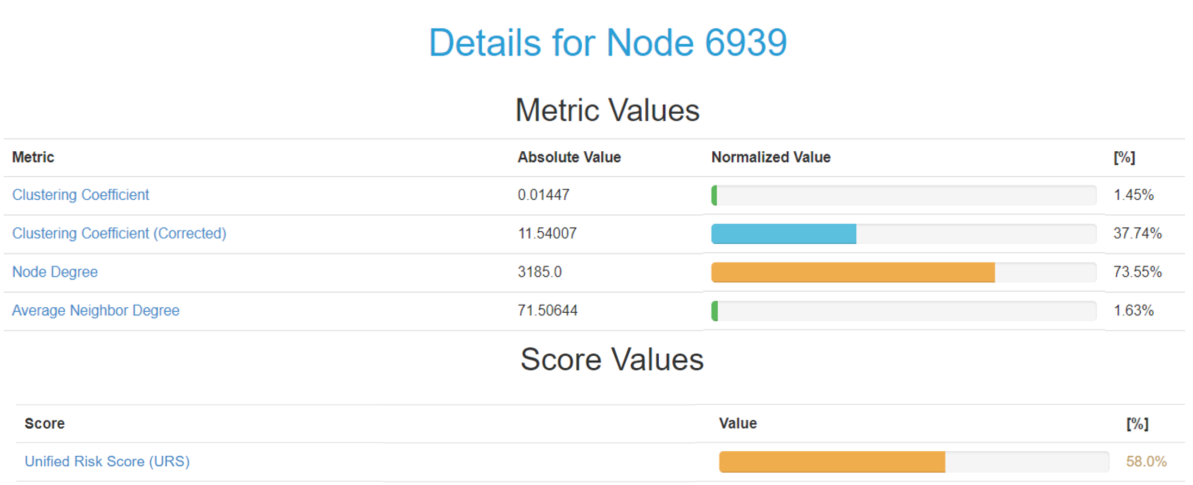
\includegraphics[scale=0.4]{Graphics/coriaExtract.PNG}}
\caption{Extract of Coria Dashboard}
\label{fig}
\end{figure}

\begin{figure}[htbp]
\centerline{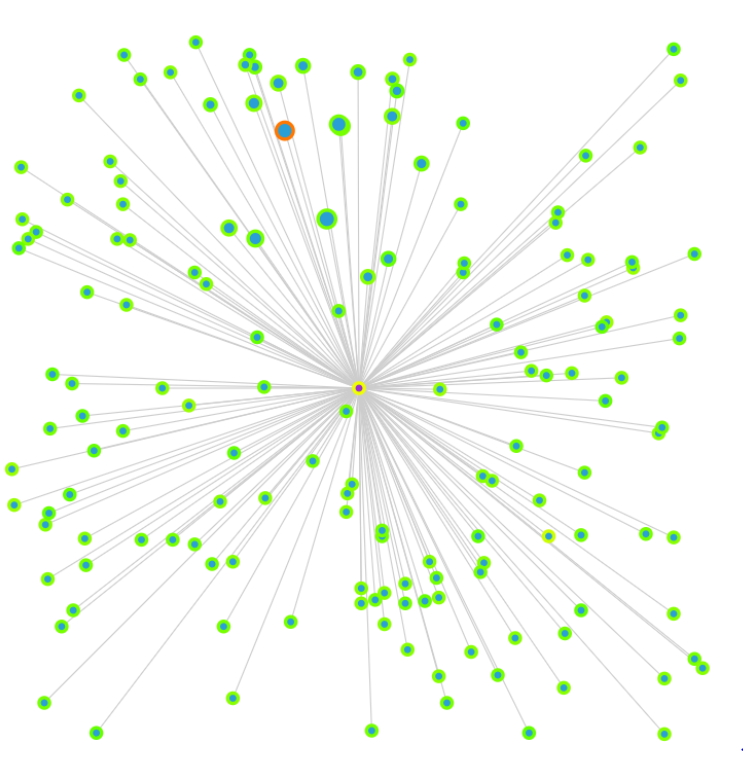
\includegraphics[scale=0.2]{Graphics/nodePresentaion.PNG}}
\caption{Graph Presentation of Nodes in a Network}
\label{fig}
\end{figure}


(old?)
Objective of our Work:
The idea is to develop systems which have the possibility to load a wide range of datasets and transform them into one standardized format which can be handled by CoRiA.
The challenge is how the large amount of different data can be transferred to make them comparable.
Another challenge is that the alternation rate of the internet graph is very fast. Millions of systems go online and others disappear day after day. So, the ETL systems have to deal with this situation as well and need to be able to load permanently new data sets.

\section{Theoretical Background}
\subsection{Autonomous Systems}

Autonomous Systems (AS) represents one level of internet topology
A set of routers under a single administration

define: AS rank, customer cone, relation ships, etc. \\


Fokussing on connectivity risks on AS-level 






\begin{figure}[htbp]
\centerline{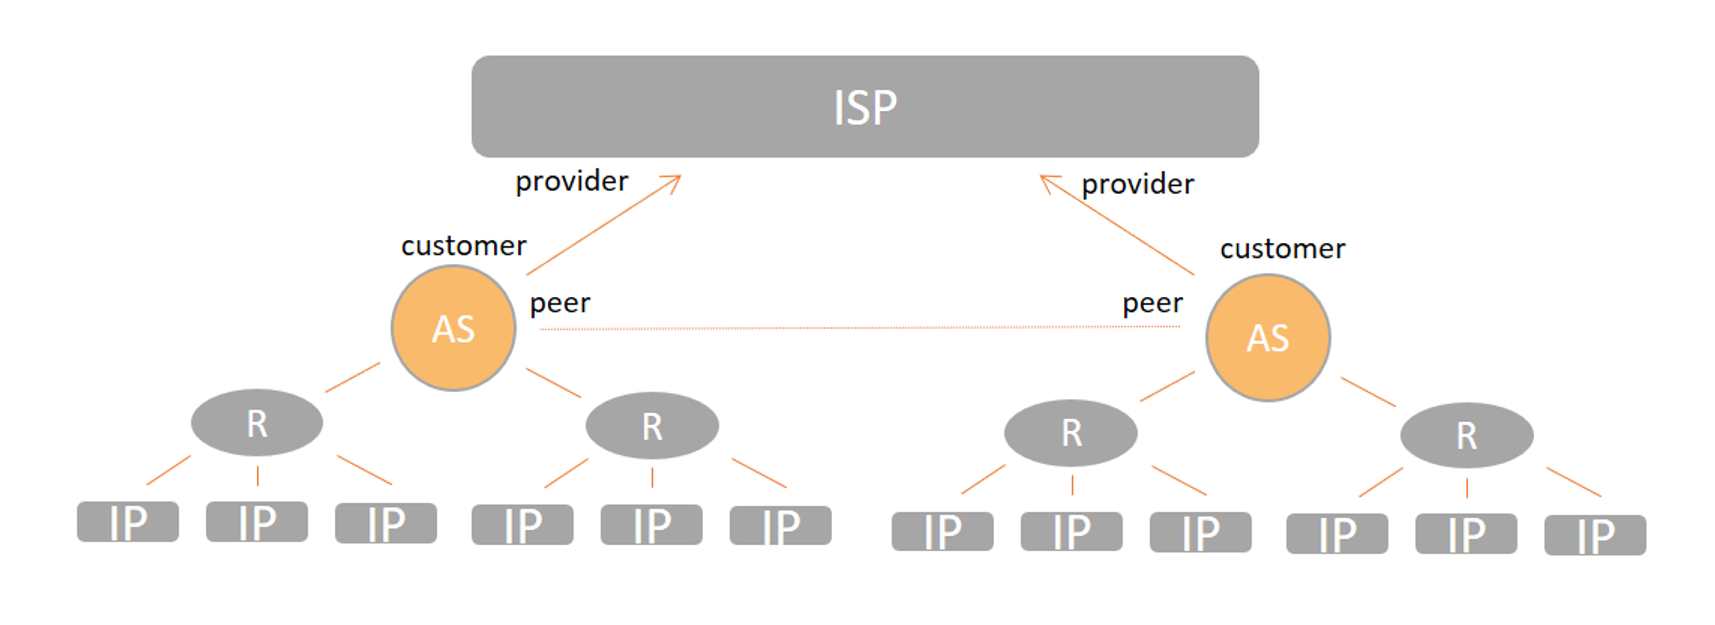
\includegraphics[scale=0.25]{Graphics/hierarchy.PNG}}
\caption{Hierarchy of the Internet}
\label{fig}
\end{figure}

\begin{figure}[htbp]
\centerline{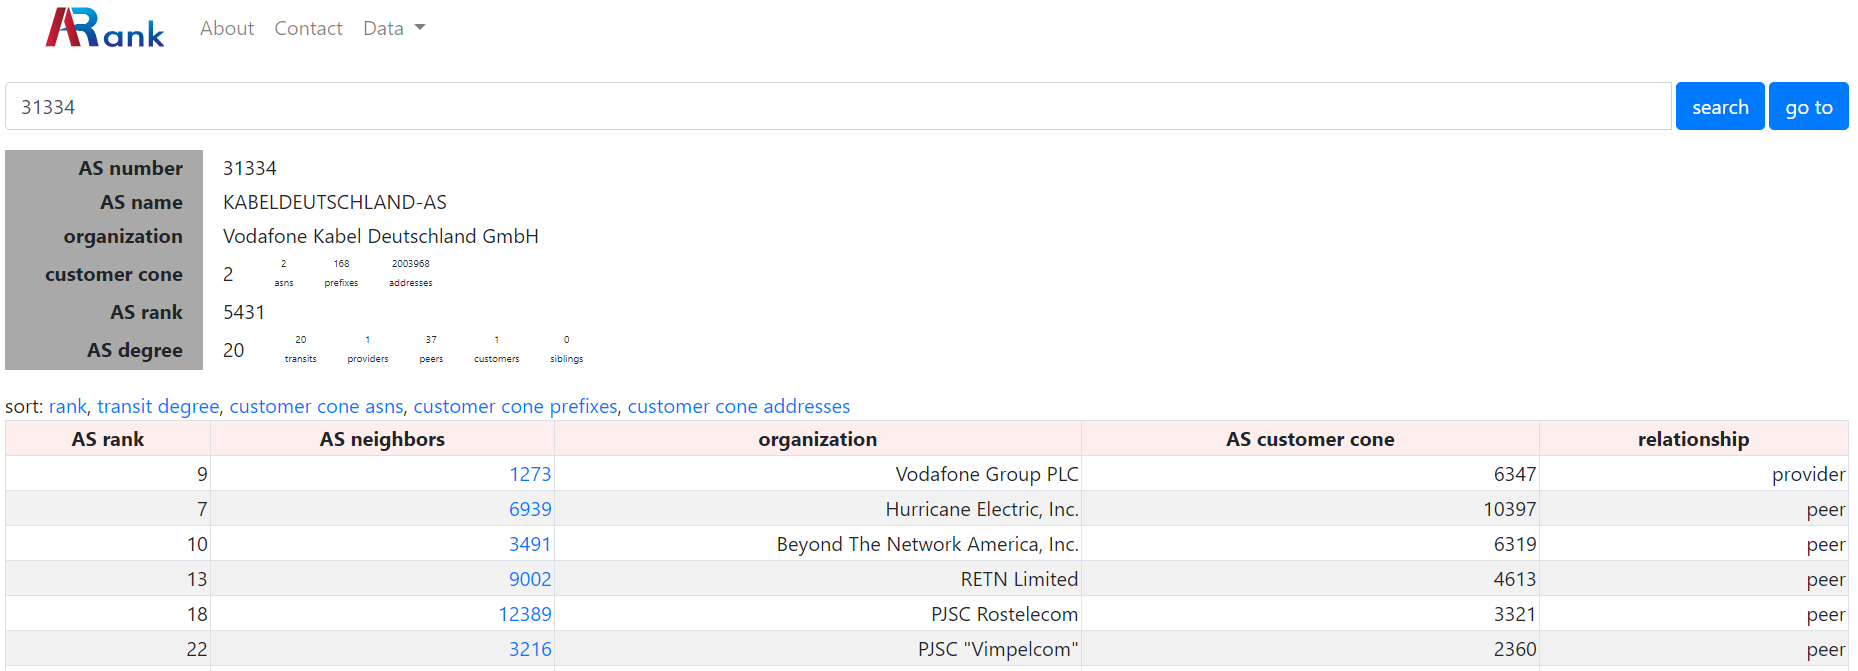
\includegraphics[scale=0.15]{Graphics/asExample.PNG}}
\caption{Example of an AS and its characteristics (Source: Caida)}
\label{fig}
\end{figure}



\subsection{ETL Process}

Extraction: from data source(s), varying data formats
Transform: convert different data into proper format, that is storable
Load: load into target database




\begin{figure}[htbp]
\centerline{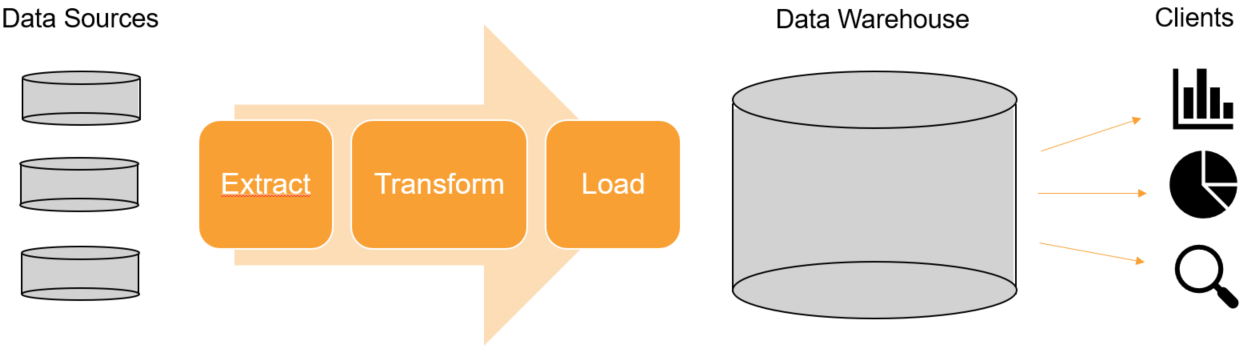
\includegraphics[scale=0.3]{Graphics/ETLTheory.PNG}}
\caption{Theoretical ETL Process}
\label{fig}
\end{figure}

\section{Data}
As a data source for this work, we exclusively focus on Caida. Caida is an appreviation and stands for Center for Applied Internet Data Analysis. Located in the San Diego, CA in the United States, the center studies networks, its infrastructure up to a large scale. For their investigation on theoretical and pracrtical aspects of the internet they monitor, collect and provide network data. 

Regarding the data granularity our primary focus lies on AS level data. Within this domain, we investigate five (?) data sets. AS-Rank offers a data base giving information about specific Autonomous Systems, like its rank, relationship to other ASes or customer cone (http://as-rank.caida.org/about) . AS Classification representa a dataset including information on the business types of Autonomous Systems. Trough machine-learning inference, Caida is able to offer this knowledge (http://www.caida.org/data/as-classification/). A dataset named Pv4 Routed 24 AS Links Dataset is used in detail to investigate the topology on the internet, its structure regarding flows of traffic, and ratios of sending and receivin autonomous systems %(http://www.caida.org/data/active/ipv4_routed_topology_aslinks_dataset.xml). 
We investigate the dataset AS Relationships in order to find out about Provider to Customer relationships as well as Peer to Peer relationships.  Lastly, we take into account geographic information of the Autonomous Systems to draw conlclusions on regions with high imapact on the internet network and less involved ones (http://www.caida.org/data/as-relationships-geo/)


For the purpose of investigating the characteristics of Ases itself and their network, we analyzed recent data of December 2017.  As part of our time series analysis, we used data from 2007 until 2017. 


\section{Results}

\subsection{Data Analysis}
First aspect of the data analysis process is the type of autonomous system. Caida distinguished here between three types: The first type are ASes that provide internets access or function as a transit. They make out 42.2\% of all nodes in the network. Second type are ASes providing content hosting and distribution systems, like Dropbox or Google, with only 4,5\% of all overall nodes. Third category are enterprises meaning organizations, universities or companies that are mostly users. They account for 53.3\%. Insights we are gaining from this aspect is that most of the nodes are representing users of the internet, which makes intuetively sense. More interesting is the large amount of transits and access points needed to provide the respective infrastructure. This hints to the internet's high complexity. 


\begin{figure}[htbp]
\centerline{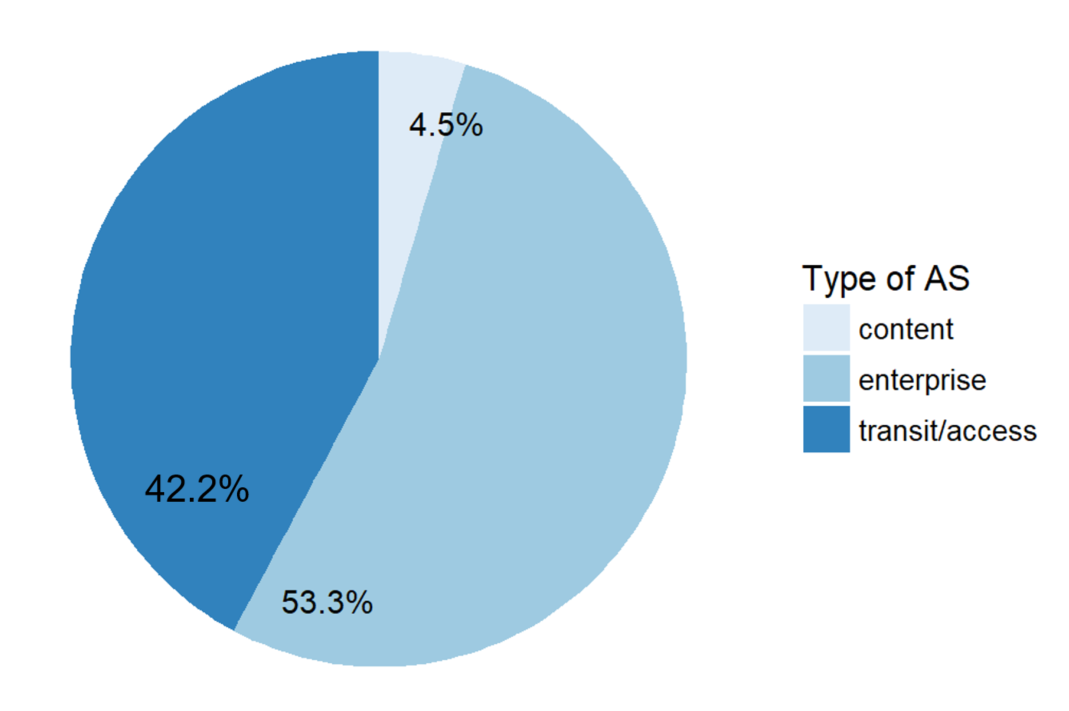
\includegraphics[scale=0.4]{Graphics/typeofAS.PNG}}
\caption{Ratio of Autonomous Systems regarding their Type }
\label{fig}
\end{figure}

As depicted in the theoretical part, autonomous systems have relationships. We took a look at this characteristic and noticed a quite balanced ratio of Provider-to-Customer relations and Peer-to-Peer relations. If we translate this into a graph, we imagine a balanced graph, which in terms of network riskiness, is rather roboust. 

\begin{figure}[htbp]
\centerline{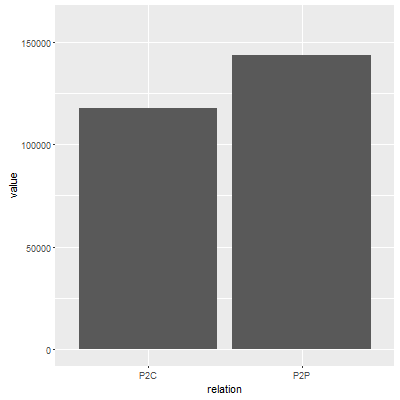
\includegraphics[scale=0.4]{Graphics/relationspeerandprovider.png}}
\caption{Ratio of AS-Relationships }
\label{fig}
\end{figure}


We furthermore built a graphs describing the distributional characteristics of autonomous systems. Figure ... shows the distribution of autonomous systems and how many outgoing connections the single nodes have. Approximately 5.500 sending nodes are containted within that data set. We ranked them on the x-axis. Wit the number of connections an AS is sending to on the y-axis, we obtrain a very left centered distribution. A very small number of nodes in the network are sending traffic to a high number of other nodes. Take the first 30 (?): ... This top ranked 30 nodes send ... \% of overall trafic of the whole network. Note that when we make statements of the whole network, we only refer to the data at hand as the whole network. That is the data collected by CAIDA. Information on CAIDA's data collection process can be found in the Appendix .. (?). 

Simultaneousely, we drew the distribution of incomming connections per Autonomous System (Appendix ...) and received a similar result. With approximately 250.000 nodes, receiving traffic, only very few nodes are receiving traffic from a high number of nodes. The top ... ranked nodes are receiving ... \% of the overall trafic in this network. 

An important finding regarding connectivity risks of the network is, how vulnerable this network is. An attack targeting the most active and most influential nodes in the network, achieving a non-functioning of those quickly leads to wide shot-downs of the network.  This again underscores the demand for Coria - a tool to analyze connectivity risks. 


\begin{figure}[htbp]
\centerline{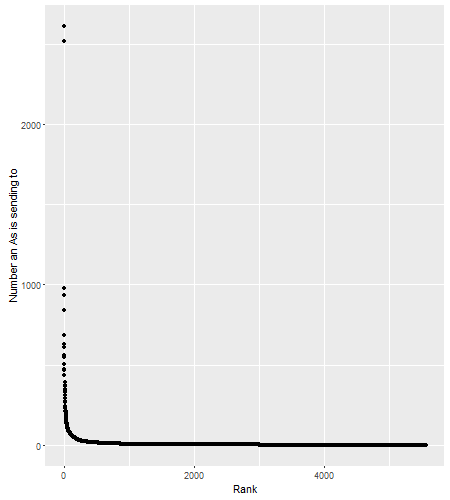
\includegraphics[scale=0.4]{Graphics/AsFromDistribution.png}}
\caption{Distribution of Outgoing Connections per AS}
\label{fig}
\end{figure}



Next, we analyzed the geographic locations of autonomous systems and their flow to traffic. Figure ... symbolizes autonomous systems as organge points on a word map. We can see a high concentration of ASes in North America and Europe. The concentration of ASes is less dense in areas like South America, Africa or Asia. Insights that we can draw from that representaion are that more autonomous systems are situated in highly developed economies  than they are in less developed regions. While we need to keep in mind that we are only analyzing one data set - with challenging data collection on top of that, we can interpret this result still as a representative sample of the overall network.(Remark: Difficult collection of AS-data and gathering through inference(?)) The results confirm the assumption that most traffic is taking place between parties of richer and more developed economies.  (auf punkte ohne verbindung hinweisen?)



\begin{figure}[htbp]
\centerline{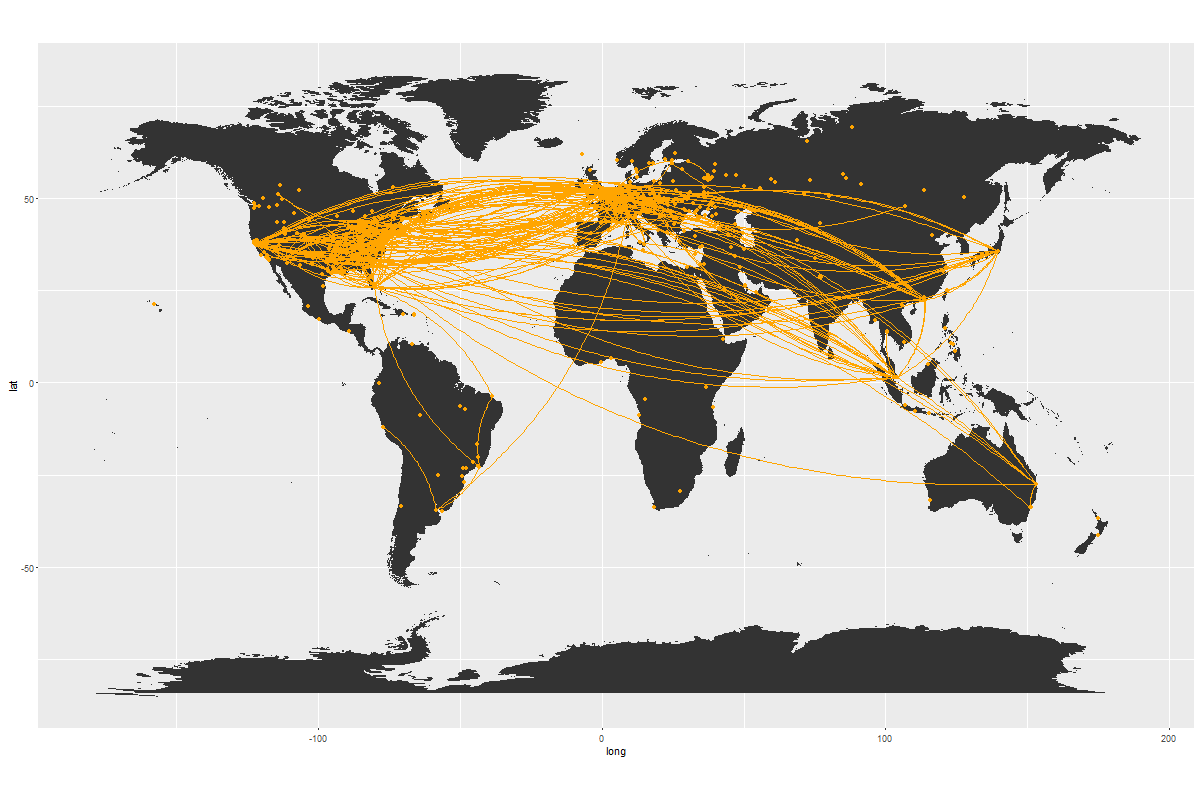
\includegraphics[scale=0.2]{Graphics/connectedASes.png}}
\caption{Location of ASes and respective Streams of traffic}
\label{fig}
\end{figure}

In addition to the analysis of a single point in time, we investigated the timely development of the network. Figure .. shows the number of traffic-sending autonomous systems from the beginning of 2007 until the end of 2017. Within these 10 years, there is a clear upward trend. In 2015 this upward trend vanishes and and reaches a constant level of approximately 5.500 sending AS nodes within the network. (Note the consistency of results with respect to Figure .. `Distribution of number of sending ASes`.) Striking in that graph are the multiple outliers appearing throught the time series. A qualitative research about exectional events happening on these dates that might have benn the reason for a downtime of multiple nodes did not lead to reasonable results. As a consequence, we assume the outliers to be caused by monitoring and data collection problems of CAIDA. (hint to appendix with data collection problem).

With respect to Appendix ..... (other time series graph) you can see a simultaneous development for the amount of nodes, receiving traffic - on a level of approx. 250.000 nodes of course. 




\begin{figure}[htbp]
\centerline{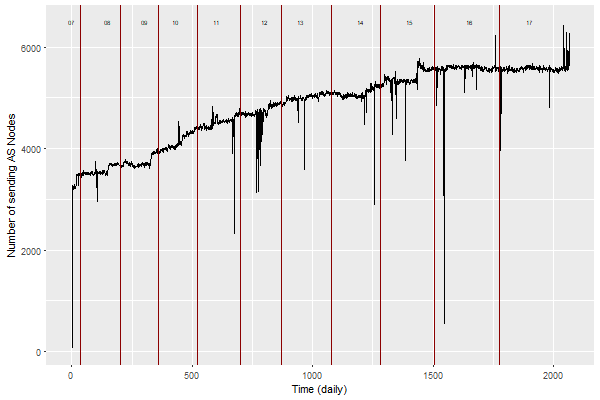
\includegraphics[scale=0.4]{Graphics/ASFromAll.png}}
\caption{Time development from 2007 - 2017: Number of sending AS nodes}
\label{fig}
\end{figure}


\subsection{Development of an automated ETL Process}

Carls part blablablabalbal



\begin{figure}[htbp]
\centerline{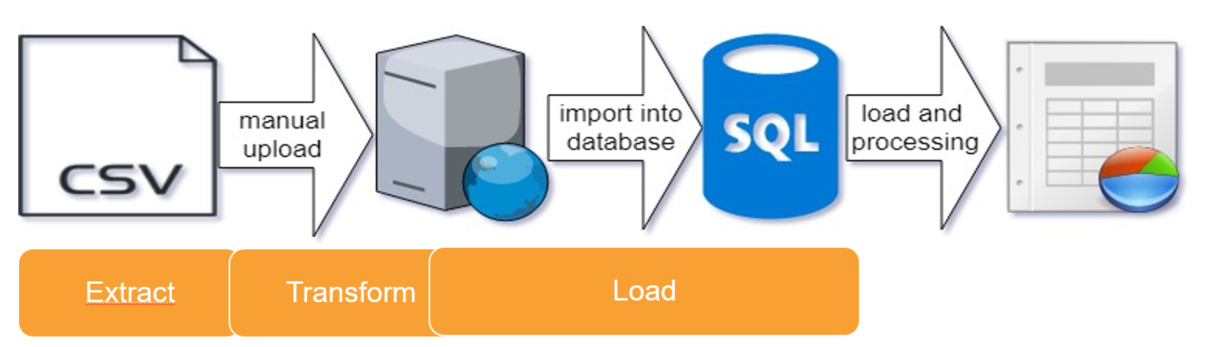
\includegraphics[scale=0.29]{Graphics/ETL1.PNG}}
\caption{A Theoretical ETL Process}
\label{fig}
\end{figure}

\begin{figure}[htbp]
\centerline{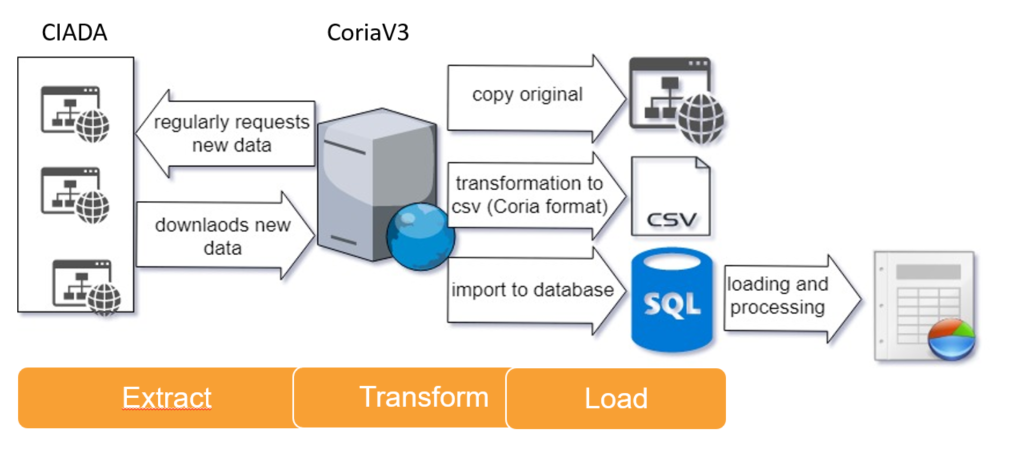
\includegraphics[scale=0.4]{Graphics/ETL2.PNG}}
\caption{ETL Process in the Coria framework}
\label{fig}
\end{figure}


\section{Conclusion} %für eine Formulierung entscheiden
\subsection{Summary}
\subsection{Limitations and Further Work}
Evaluation: \\
Validation of latest data files

Copy of current data files

Transformion data to csv

Import data into the Coria MySQL database

Import scripts to the Coria framework (Python -> Java)

Data aggregation over time

Outlook:\\
Apply automated ETL process to further data sources
Run Coria on a server (longtime evaluation)
Documentation


\begin{thebibliography}{00}


\bibitem{b1}still old!noch die aus der Präsi einfügen'! G. Eason, B. Noble, and I. N. Sneddon, ``On certain integrals of Lipschitz-Hankel type involving products of Bessel functions,'' Phil. Trans. Roy. Soc. London, vol. A247, pp. 529--551, April 1955.
\bibitem{b2} J. Clerk Maxwell, A Treatise on Electricity and Magnetism, 3rd ed., vol. 2. Oxford: Clarendon, 1892, pp.68--73.
\bibitem{b3} I. S. Jacobs and C. P. Bean, ``Fine particles, thin films and exchange anisotropy,'' in Magnetism, vol. III, G. T. Rado and H. Suhl, Eds. New York: Academic, 1963, pp. 271--350.
\bibitem{b4} K. Elissa, ``Title of paper if known,'' unpublished.
\bibitem{b5} R. Nicole, ``Title of paper with only first word capitalized,'' J. Name Stand. Abbrev., in press.
\bibitem{b6} Y. Yorozu, M. Hirano, K. Oka, and Y. Tagawa, ``Electron spectroscopy studies on magneto-optical media and plastic substrate interface,'' IEEE Transl. J. Magn. Japan, vol. 2, pp. 740--741, August 1987 [Digests 9th Annual Conf. Magnetics Japan, p. 301, 1982].
\bibitem{b7} M. Young, The Technical Writer's Handbook. Mill Valley, CA: University Science, 1989.
\end{thebibliography}


\appendix

Nummerierung vom Appendix stimmt noch nicht

\section{\\Distribution of Incoming Connections per AS}


\begin{figure}[htbp]
\centerline{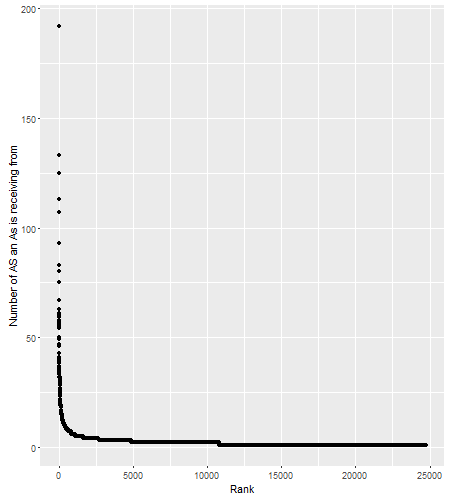
\includegraphics[scale=0.4]{Graphics/AsToDistribution.png}}
\caption{Distribution of Incoming Connections per AS}
\label{fig}
\end{figure}


Geographical Locations of ASes
\section{\\Geographical Locations of ASes}
\begin{figure}[htbp]
\centerline{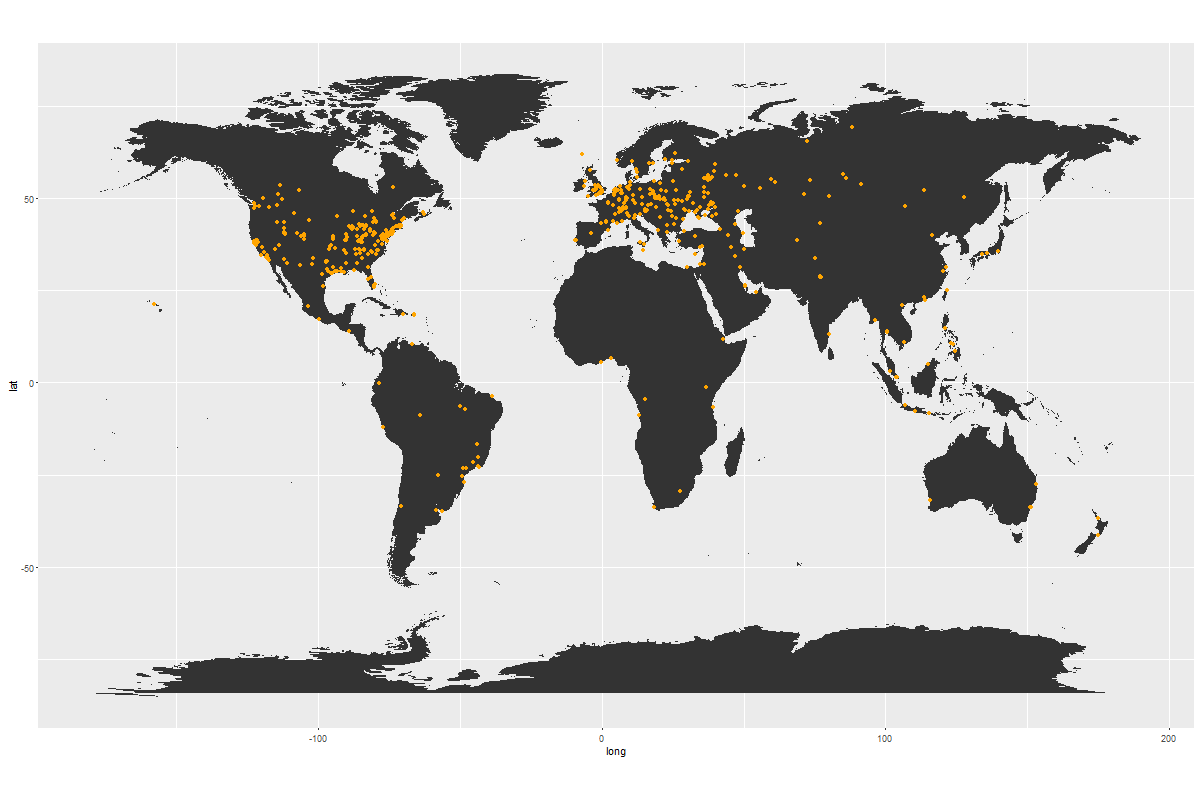
\includegraphics[scale=0.2]{Graphics/ASesNurPunkte.png}}
\caption{Geographical Locations of ASes}
\label{fig}
\end{figure}


Time development from 2007 - 2017: Number of receiving AS nodes

\begin{figure}[htbp]
\centerline{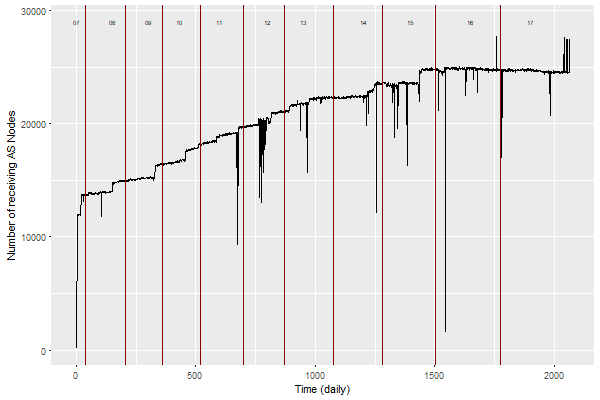
\includegraphics[scale=0.4]{Graphics/ASToAll.png}}
\caption{Time development from 2007 - 2017: Number of receiving AS nodes}
\label{fig}
\end{figure}




\section{\\Data Collection Process of CAIDA}
Data Collection Process of CAIDA





\end{document}
